\documentclass[xcolor=dvipsnames,aspectratio=169,t]{beamer}
  % t means frames are vertically centered to the top
\usepackage{slides-header}
\title{Coordinate Systems}

% This slide needs to be fixed.  Too much emphasis on the change of basis matrix to the standard basis.  Weird.

\begin{document}
\maketitle

\begin{frame}{Basis of a Vector Space}
  \medskip

  Recall:
  \bbox
  Let $H$ be a subspace of a vector space $V$. A set $\mathcal{B}$ of vectors in $V$ is a \alert{basis for $H$} if:
  \begin{itemize}
  \item $\mathcal{B}$ is a \alert{linearly independent set}, and
  \item the subspace spanned by $\mathcal{B}$ equals $H$ (ie, \alert{$\mbox{Span } \mathcal{B} = H$}).
  \end{itemize}
  \ebox
\end{frame}

\begin{frame}{The Uniqueness Representation Theorem}

{\small One nice result of choosing a basis $\mathcal{B}$ for a vector space $V$ is to impose a \alert{coordinate system} on $V$.}

  \begin{example}
  {\small 
  \begin{itemize}
  \item
  If $V = \mathbb{R}^4$ with standard basis 
  $\mathcal{B} = \left\{ \e_1, \e_2, \e_3, \e_4 \right\}$, then
  \[ \begin{bmatrix} 2 \\ -5 \\ 17 \\ -8 \end{bmatrix} = 2 \e_1 - 5 \e_2 + 17  \e_3 - 8  \e_4.\]
  
  \item 
  Consider the vector space $V = \mbox{Mat}_{2 \times 2}$ and the basis $\dsty \mathcal{B} = \left\{ \begin{bmatrix} 1 & 0 \\ 0 & 0 \end{bmatrix} , \begin{bmatrix} 0 & 1 \\ 0 & 0 \end{bmatrix} ,  \begin{bmatrix} 0 & 0 \\ 1 & 0 \end{bmatrix} ,  \begin{bmatrix} 0 & 0 \\ 0 & 1 \end{bmatrix} \right\}$.

  Then an element in $\mbox{Mat}_{2 \times 2}$ such as $\begin{bmatrix} 2 & -5 \\ 17 & -8 \end{bmatrix}$ can be written as the linear combination:
  \[ \begin{bmatrix} 2 & -5 \\ 17 & -8 \end{bmatrix} = 2 \v_1 -5  \v_2 + 17 \v_3 -8 \v_4. \]

  \end{itemize}
  }
  \end{example} 

\end{frame}

\begin{frame}{The Uniqueness Representation Theorem}
  \begin{theorem}
  Let $\B = \left\{ \b_1,\b_2,\ldots,\b_n \right\}$ be a basis for a vector space $V$.
  Then for each $\x$ in $V$, there exists a \alert{unique set of scalars} $c_1, c_2, \ldots, c_n$ (our coordinates) such that
  \begin{equation}
  \x = c_1 \b_1 + c_2 \b_2 + \ldots + c_n \b_n.
  \end{equation}
  \end{theorem}

  \pause
  \blue{Proof.}
  Since $\B$ spans $V$, we know there exists scalars such that equation (1) above holds. Suppose the representation is not unique, and there exist scalars $d_1, d_2, \ldots , d_n$ such that
  \[ \x = d_1 \b_1 + d_2 \b_2 + \ldots + d_n \b_n.\]
  \vspace*{-2.5em}
  
  \pause
  Subtracting the two gives
  \begin{equation}
  \mathbf{0} = (c_1 - d_1) \b_1 +  (c_2 - d_2) \b_2 +  \ldots +  (c_n - d_n) \b_n.
  \end{equation}
  Since we assumed $\mathcal{B}$ is a basis for $V$, equation (2) has only the trivial solution, so $c_j=d_j$ for all $1 \leq j \leq n$.
  Thus we see the representation is \alert{unique}.
  \hfill\blue{\qed}
\end{frame}


\begin{frame}{Coordinates Relative to a Basis}
  \begin{definition}
  Suppose $\B = \left\{ \mathbf{b}_1,  \mathbf{b}_2, \ldots ,  \mathbf{b}_n \right\}$ is a basis for a vector space $V$, and $\mathbf{x}$ is in $V$. The \alert{coordinates of $\mathbf{x}$ relative to the basis $\B$} (or the \alert{$\B$-coordinates of $\mathbf{x}$}) are the unique scalars $c_1, c_2, \ldots , c_n$ such that $\mathbf{x} = c_1 \mathbf{b}_1 + c_2 \mathbf{b}_2 + \ldots + c_n \mathbf{b}_n$.
  \end{definition}

\begin{definition}
If $c_1, c_2, \ldots , c_n$  are the $\B$-coordinates of $\mathbf{x}$, then the vector in $\mathbb{R}^n$
\[ \lbrack \mathbf{x} \rbrack_{\B} = \begin{bmatrix} c_1 \\ c_2 \\ \vdots \\ c_n \end{bmatrix} \]
is the \alert{$\B$-coordinate vector of $\mathbf{x}$}.
\end{definition}

\end{frame}


\begin{frame}{Mapping $V$ to $\mathbb{R}^n$}

\begin{definition}
The mapping $V \to \mathbb{R}^n: \mathbf{x} \mapsto \lbrack \mathbf{x} \rbrack_{\B}$ is the \alert{coordinate mapping} (determined by $\B$).
\end{definition}



\[ \colorb{\mbox{Mat}_{2 \times 2}} \to \alert{\mathbb{R}^4}: \colorb{\begin{bmatrix} 2 & -5  \\ 17 & -8 \end{bmatrix}} \mapsto \alert{\begin{bmatrix} 2 \\ -5 \\ 17 \\ -8 \end{bmatrix}} \]

\end{frame}

\begin{frame}{Example}

\begin{columns}[t]

\column{0.3\tw}

Let $V = \mathbb{R}^2$ and consider the vector $\mathbf{x} = \begin{bmatrix} 3 \\ -5 \end{bmatrix}$.

\column{0.7\tw}

Consider two different bases for $V$:
\[ \alert{\B_1 = \left\{ \begin{bmatrix} 1 \\ 0 \end{bmatrix} , \begin{bmatrix} 0 \\ 1 \end{bmatrix} \right\}} \quad \mbox{and} \quad \colorb{ \B_2 = \left\{ \begin{bmatrix} 1 \\ -1 \end{bmatrix} , \begin{bmatrix} 1 \\ 1 \end{bmatrix} \right\}} \]

\end{columns}

\pause
\begin{columns}[t]

  \column{0.3\tw}
    We have  $\mathbf{x} = 3 \mathbf{e}_1 -5 \mathbf{e}_2$, so
    \alert{\[ \lbrack \mathbf{x} \rbrack_{\B_1} = \begin{bmatrix} 3 \\ -5 \end{bmatrix}.\]}

  \column{0.7\tw}
  \medskip

  {\small
  We solve the vector equation $c_1 \begin{bmatrix} 1 \\ -1 \end{bmatrix} + c_2 \begin{bmatrix} 1 \\ 1 \end{bmatrix} = \begin{bmatrix} 3 \\ -5 \end{bmatrix}$.
  \medskip

  This system of linear equations has augmented matrix
  \[ \begin{bmatrix} 1 & -1 & 3\\ -1 & 1 & -5 \end{bmatrix} \sim \begin{bmatrix} 1 & 0 & 4\\ 0 & 1 & -1 \end{bmatrix} \]

  Thus we have \colorb{$\dsty \lbrack \mathbf{x} \rbrack_{\B_2} = \begin{bmatrix} 4 \\ -1 \end{bmatrix}$} since 
  $\dsty \mathbf{x} = \begin{bmatrix} 3 \\ -5 \end{bmatrix} = 4 \begin{bmatrix} 1 \\ -1 \end{bmatrix} -1  \begin{bmatrix} 1 \\ 1 \end{bmatrix}$.
  }
  \end{columns}
\end{frame}

\begin{frame}{Geometric Interpretation}
  Let $V = \mathbb{R}^2$ and consider the vector $\mathbf{x} = \begin{bmatrix} 3 \\ -5 \end{bmatrix}$.
  \medskip

  Consider two different bases for $V$:
  $\dsty \alert{\B_1 = \left\{ \begin{bmatrix} 1 \\ 0 \end{bmatrix} , \begin{bmatrix} 0 \\ 1 \end{bmatrix} \right\}}$ and $\dsty \colorb{ \B_2 = \left\{ \begin{bmatrix} 1 \\ -1 \end{bmatrix} , \begin{bmatrix} 1 \\ 1 \end{bmatrix} \right\}}$.

\begin{columns}[T]

  \column{0.6\tw}

  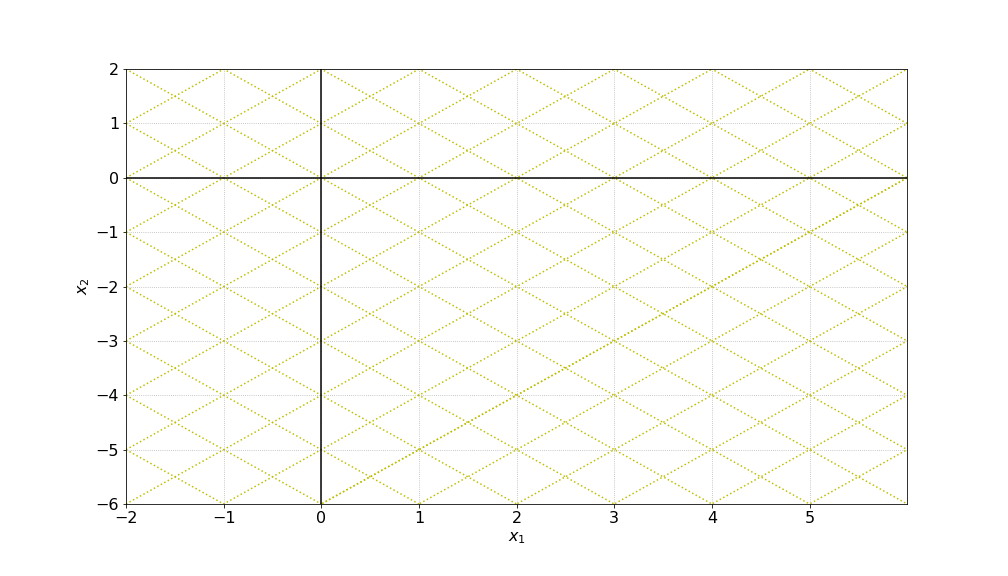
\includegraphics[width=0.99\tw]{images/fig-diff-basis.png}

\column{0.4\tw}

\vspace{0.2in}

We have \alert{$\begin{bmatrix} 3 \\ -5 \end{bmatrix} = 3 \begin{bmatrix} 1\\ 0 \end{bmatrix} - 5 \begin{bmatrix} 0\\ 1 \end{bmatrix}$}.

\alert{$\lbrack \mathbf{x} \rbrack_{\B_1} = \begin{bmatrix} 3 \\ -5 \end{bmatrix}$} \bs

We have \colorb{$\begin{bmatrix} 3 \\ -5 \end{bmatrix} = 4 \begin{bmatrix} 1\\ -1 \end{bmatrix} -1 \begin{bmatrix} 1\\ 1 \end{bmatrix}$}.

\colorb{$\lbrack \mathbf{x} \rbrack_{\B_2} = \begin{bmatrix} 4 \\ -1 \end{bmatrix}$}

\end{columns}
  
\end{frame}


%%%%%%%%%%%%%%%%%%%%%%%%%%%%%%%%%%%%%%%%%%%%%%%%%%%%%%%%%%%%%%%%%%%%%%%%%%%%%%%%%%%%%%%%%
\begin{frame}{Change of Coordinates Matrix for Basis in $\mathbb{R}^n$}
  \smallskip

  Let $V = \mathbb{R}^2$  and consider the basis  $\B = \left\{ \begin{bmatrix} 1 \\ -2 \end{bmatrix} , \begin{bmatrix} -3 \\ 4 \end{bmatrix} \right\}$.
  \smallskip

  Suppose vector $\x$ in $\mathbb{R}^2$ has $\B$-coordinates
  $\lbrack \x \rbrack_{\B} = \begin{bmatrix} 2 \\ -6 \end{bmatrix}$.
  \smallskip
  
  \alert{How can we determine what the coordinates of this vector are in the standard basis?}

  \pause
  \[ 2 \begin{bmatrix} 1 \\ -2 \end{bmatrix} -6 \begin{bmatrix} -3 \\ 4 \end{bmatrix}  = \colorb{\begin{bmatrix} 1 & -3 \\ -2 & 4 \end{bmatrix}} \begin{bmatrix} 2 \\ -6 \end{bmatrix} = \begin{bmatrix} 20 \\ -28 \end{bmatrix} \]

  \pause
  The matrix $\colorb{P = \begin{bmatrix} 1 & -3 \\ -2 & 4 \end{bmatrix} = \begin{bmatrix} \b_1 & \mathbf{b_2} \end{bmatrix}}$ is called the \colorb{change of coordinates matrix from $\B$ to the standard basis} in $\mathbb{R}^2$.
  \medskip

  In general, if $\B = \left\{ \b_1 ,  \b_2, \ldots ,  \b_n \right\}$ is a basis for $\R^n$, then the \alert{change of coordinates matrix from $\B$ to the standard basis} in $\R^n$ is given by the matrix \alert{$P_{\B} = \begin{bmatrix} \b_1 &  \b_2 & \ldots & \b_n \end{bmatrix}$}.

\end{frame}

\begin{frame}

Let $V = \mathbb{R}^2$  and consider the basis  $\B = \left\{ \begin{bmatrix} 1 \\ -2 \end{bmatrix} , \begin{bmatrix} -3 \\ 4 \end{bmatrix} \right\}$.

Let $\mathbf{x} = \begin{bmatrix} 8 \\ -11 \end{bmatrix}$. Find the $\B$-coordinates of $\mathbf{x}$.

\pause
\bi
\ii We have the change of coordinate matrix \colorb{$P = \begin{bmatrix} 1 & -3 \\ -2 & 4 \end{bmatrix}$} which maps $\lbrack \mathbf{x} \rbrack_{\B}$ to the standard basis. 
\ii We want to do the inverse of this map (map standard basis to $\lbrack \mathbf{x} \rbrack_{\B}$).
\ii The inverse matrix $P^{-1}$ of $P$ will do the job.
\ei

\pause
In this example, we have

\[ \colorb{P = \begin{bmatrix} 1 & -3 \\ -2 & 4 \end{bmatrix}} \quad \mbox{and} \quad \alert{P^{-1} = \begin{bmatrix} -2 & -1.5 \\ -1 & -0.5\end{bmatrix}}. \]

This gives

\[ \lbrack \mathbf{x} \rbrack_{\B} = \alert{P^{-1}} \mathbf{x} =  \alert{\begin{bmatrix} -2 & -1.5 \\ -1 & -0.5\end{bmatrix}} \begin{bmatrix} 8 \\ -11 \end{bmatrix} = \begin{bmatrix} 0.5 \\ -2.5 \end{bmatrix}. \]
\end{frame}


\begin{frame}{Coordinate Mappings from $V$ into $\mathbb{R}^n$}
  \bigskip

  Given a vector space $V$ with basis $\B = \left\{ \mathbf{b}_1 ,  \mathbf{b}_2 , \ldots ,  \mathbf{b}_n \right\} $, we can define the coordinate map

  \[ T: V \to \mathbb{R}^n: \mathbf{x} \mapsto \lbrack \mathbf{x} \rbrack_{\B}.\]
  \vspace*{-1em}  % so weird

  \bbox
  The coordinate mapping above is a \alert{one-to-one} linear transformation from $V$ \alert{onto} $\mathbb{R}^n$. 

  A linear transformation that is \colorr{both} one-to-one and onto is called an \alert{isomorphism}.
  \ebox
  \bigskip
  
  Thus, $V$ and $\R^n$ have the ``\blue{same shape}'' with respect to vector space properties (ie, vector addition and scalar multiplication).
\end{frame}


\begin{frame}{Example}
  \bigskip

  Let $V = \mathbb{P}_3$ with basis $\B = \left\{ 1, t, t^2, t^3 \right\}$. 
  Then the coordinate mapping onto $\mathbb{R}^4$ is given by

  \[ T(1) = \mathbf{e}_1 , T(t) = \mathbf{e}_2 ,T(t^2) = \mathbf{e}_3 , \mbox{ and } T(t^3) = \mathbf{e}_4.\]
  \bigskip

  \colorb{Find the $\B$-coordinates of the vector (polynomial) $\mathbf{x} = 2+2t^2-5t^3$.}
  \bigskip

  \pause
  We have $T(\mathbf{x}) = T(\alert{2} + \alert{0}t + \alert{2}t^2-\alert{5}t^3)= \alert{2} \mathbf{e}_1 + \alert{0}  \mathbf{e}_2+ \alert{2}  \mathbf{e}_3 \alert{- 5} \mathbf{e}_4  $, which gives \alert{$ \lbrack \mathbf{x} \rbrack_{\B} = \begin{bmatrix} 2\\ 0 \\ 2 \\ -5 \end{bmatrix}$}.
\end{frame}


\begin{frame}%{Coordinate System for a Polynomial Vector Space}

  Let $V = \mathbb{P}_3$ with basis $\B = \left\{ 1, t, t^2, t^3 \right\}$.
  Determine whether polynomials 
  $\v_1 = 2+2t^2-5t^3$, $\v_2 =5+t^3$, $\v_3 = 7t - 3t^2$, and $\v_4= -1 + 7t + t^2-11t^3$ form a linearly independent set.

  \vspace{0.15in}

  \pause
  We have
  $\dsty 
  \lbrack \v_1 \rbrack_{\B} = \begin{bmatrix} 2\\ 0 \\ 2 \\ -5 \end{bmatrix}, \ 
  \lbrack \v_2 \rbrack_{\B} = \begin{bmatrix} 5 \\ 0 \\ 0 \\ 1 \end{bmatrix}, \ 
  \lbrack \v_3 \rbrack_{\B} = \begin{bmatrix} 0 \\ 7 \\ -3 \\ 0 \end{bmatrix}, \ 
  \lbrack \v_4 \rbrack_{\B} = \begin{bmatrix} -1 \\ 7 \\ 1 \\ -11 \end{bmatrix}$.
  \medskip
  
  Since $\mathbb{P}_3$ and $\R^4$ are \blue{isomorphic},
  
  $\{\v_1,\v_2,\v_3,\v_4\}$ is lin indep in $\mathbb{P}_3$
  \alert{if and only if}
  $\left\{[\v_1]_\B,[\v_2]_\B,[\v_3]_\B,[\v_4]_\B\right\}$ is lin indep in $\R^4$.
  
  %\vspace{-0.1in}

  \pause
  \begin{columns}[t]
  \column{0.45\tw}

  $\begin{bmatrix} 2 & 5 & 0 & -1 \\ 0 & 0 & 7 & 7 \\ 2 & 0 & -3 & 1 \\ -5 & 1 & 0 & -11 \end{bmatrix} \sim 
  \begin{bmatrix} 1 & 0 & 0 & \colorb{2} \\ 0 & 1 & 0 &  \colorg{-1} \\ 0 & 0 & 1 &\alert{1} \\ 0 & 0 & 0 & 0 \end{bmatrix}$

  \column{0.5\tw}
  
  \vspace*{1em}
  
  Setting the free variable $x_4=1$, we obtain:
  
  $\blue{-2}[\v_1]_\B + \green{1}[\v_2]_\B \red{-1}[\v_3]_\B + 1[\v_4]_\B = \mathbf{0}$.
  \end{columns}

  \bs

  So we have $\colorb{-2} (2+2t^2-5t^3)  +  \colorg{1}(5+t^3) \alert{-1} (7t - 3t^2)
    +1(-1 + 7t + t^2-11t^3) = 0$.
\end{frame}

% skip until change of basis 
% \begin{frame}%{Example}
%   Let $V = \mathbb{P}_2$ with standard basis $\B=\{1,t,t^2\}$ 
%   and basis $\B_2 = \left\{ 1-t+t^2 , 3t+t^2, 2-t \right\}$. 
%   Find the $\B_2$-coordinates of the vector $\x = -1 + t + t^2$.
% 
%   \pause
%   \bi
%   \ii Using the standard basis for $\mathbb{P}_2$, 
%     we have $[-1 + t + t^2]_\B = \begin{bmatrix} -1 \\ 1 \\ 1 \end{bmatrix}$.
%   \ii The change of coordinates matrix from $\B_2$ to the standard basis $\B$ in $\mathbb{P}_2$ is given by the matrix 
%   \[ P_{\B_2} = \begin{bmatrix} \b_1 & \b_2 & \ldots & \b_n \end{bmatrix} =
%   \begin{bmatrix} 1 & 0 & 2 \\ -1 & 3 & -1 \\ 1 & 1 & 0 \end{bmatrix}.\]
%   \ii The change of coordinates matrix from the standard basis $\B$ in $\mathbb{P}_2$ to $\B_2$ is given by the inverse:
%   \[ \lbrack -1 + t + t^2 \rbrack_{\B_2} = \frac{1}{7} \begin{bmatrix} -1 & -2 & 6 \\ 1 & 2 & 1 \\ 4 & 1 & -3 \end{bmatrix} \begin{bmatrix} -1 \\ 1 \\ 1 \end{bmatrix} = \begin{bmatrix} 5/7 \\ 2/7 \\ -6/7 \end{bmatrix}.\]
%   \ei
% \end{frame}

\end{document}


